\chapter{Figures and tables}


%
%
%
\section{Embedding pictures}\label{sec:pictures}

Before we go into the details of figure environments,
let us first recall the syntax for embedding pictures
and some good practices.\index{pictures}

\TeX{} does not natively understand picture files;
instead, they are placed with cooperation between the \pkg{graphicx} package
and the particular \LaTeX{} compiler (pdfLaTeX or friends).

\begin{warning}
Again, careful with the spelling!
The \pkg{graphicx} package replaces the old \obspkg{graphics} package,
which has similar basic syntax but less flexibility.
\end{warning}

The basic command is \cmd{includegraphics}.
It takes the path (relative to source file) of the picture file,
and some optional arguments that we describe below.
On Linux file paths are case-sensitive, so be careful with the spelling
(otherwise your file will compile only on case-insensitive systems like Windows and macOS).
Only \verb|/| can be used as the directory delimiter.
The file extension (here \verb|.jpg|) is optional.

\begin{VerbatimOut}{\jobname.tmp}
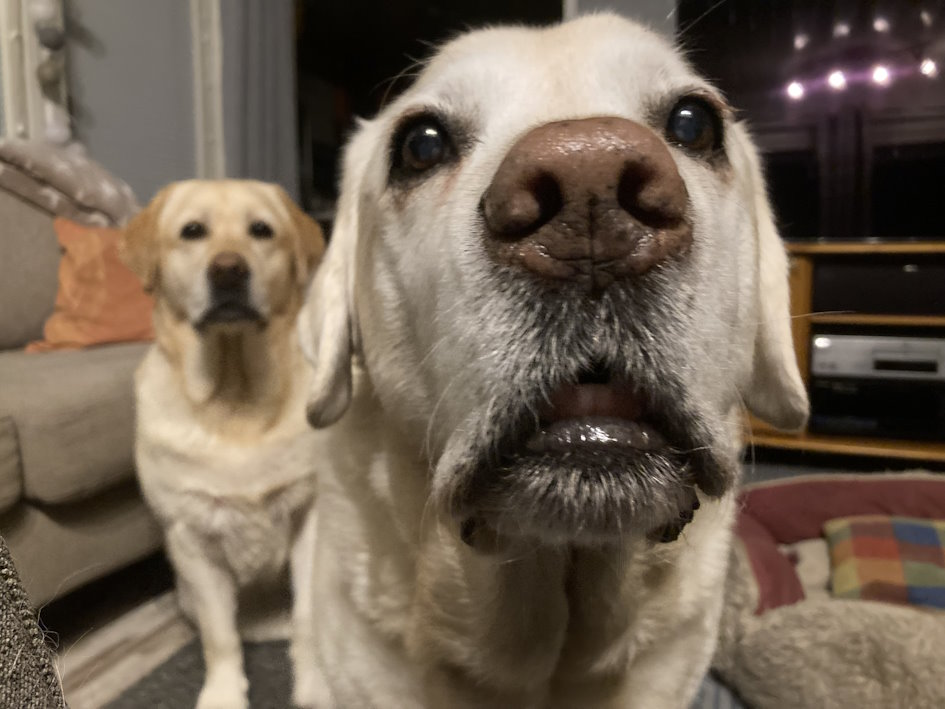
\includegraphics[width=\textwidth]
    {pictures/TheDogs.jpg}
\end{VerbatimOut}
\ShowExample

There are quite a few optional parameters using the key=value syntax:

\begin{description}
\item[width] Sets the width of the picture in document units.
    Can be any expression like \verb|width=0.5\textwidth| or \verb|width=8cm|.
    Height of the picture is chosen to match the aspect ratio.
\item[height] Alternatively, the height can be fixed and width chosen automatically.
    If both \verb|height| and \verb|width| are set,
    then the picture is \emph{stretched} to the given height and width.
\item[angle] Rotation (in degrees counterclockwise).
    The \verb|totalheight| option can be set to restrict the height of the final rotated image.
\item[origin] Origin for the rotation.
    Most useful value is \verb|c| for center;
    others are \verb|l| for left, \verb|r| for right,
    \verb|t| for top, \verb|b| for bottom, and combinations of the five.
\item[bb, clip] Named for ``bounding box'', the \verb|bb| parameter defines
    the region of the image to use in size computations.
    The \verb|clip| option then crops the image to this size.
    If this option is not set, then the image extends outside the region reserved for it!

    The bounding box is specified as \verb|bb=1 2 3 4|; in this example
    the lower-left corner is at $(1,2)$ and the upper-right at $(3,4)$,
    and the origin $(0,0)$ is at the lower-left corner of the image.
    By default the unit is ``big points'' (1/72\textsuperscript{th} of an inch),
    but other \TeX{} length units can be used.
    Due to the choice of units, this is most useful with PDF images.
\item[draft] This is usually passed as a package or document class option.
    It suppresses the inclusion of pictures into the final output;
    only boxes of the correct size are included.
    (The size computation requires the picture file to exist!)
\item[\dots] and some more can be found in the package documentation.
    I would, however, do any complicated graphical things in a proper graphics editor.
\end{description}

\begin{VerbatimOut}{\jobname.tmp}
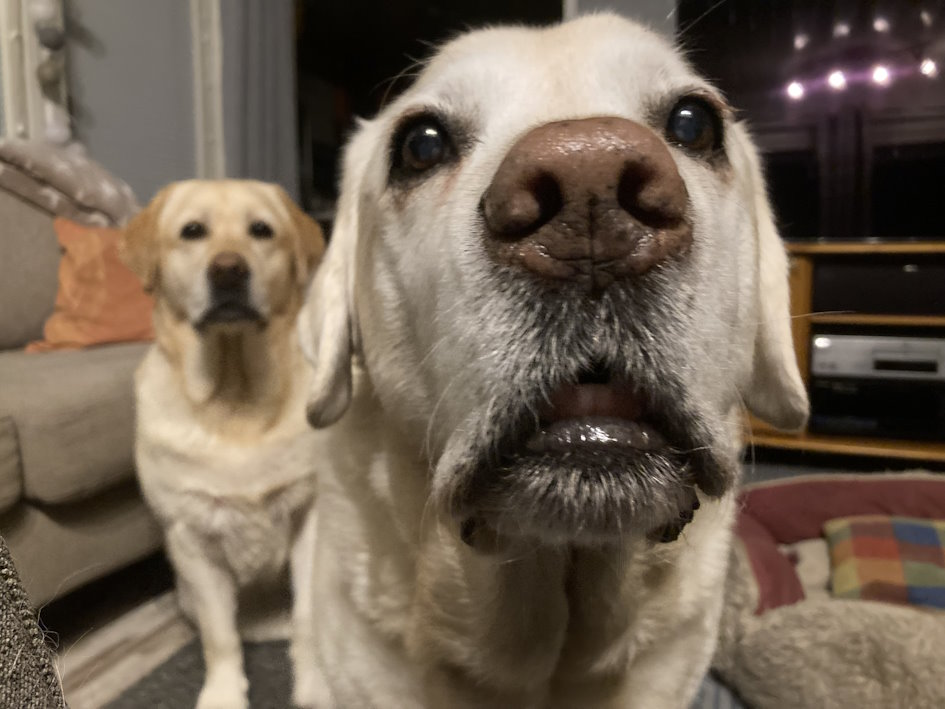
\includegraphics[bb=2.3cm 1.4cm 7cm 6cm,clip]
    {pictures/TheDogs.jpg}
\end{VerbatimOut}
\ShowExample
%
\begin{VerbatimOut}{\jobname.tmp}
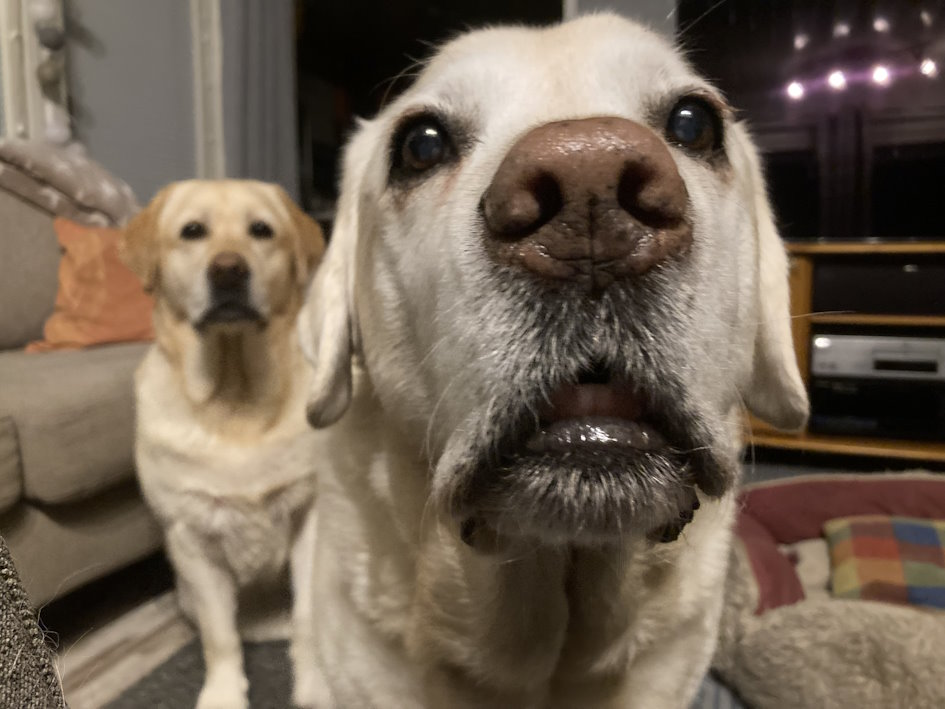
\includegraphics[totalheight=3cm, angle=45]
    {pictures/TheDogs.jpg}
\end{VerbatimOut}
\ShowExample
%
\begin{VerbatimOut}{\jobname.tmp}
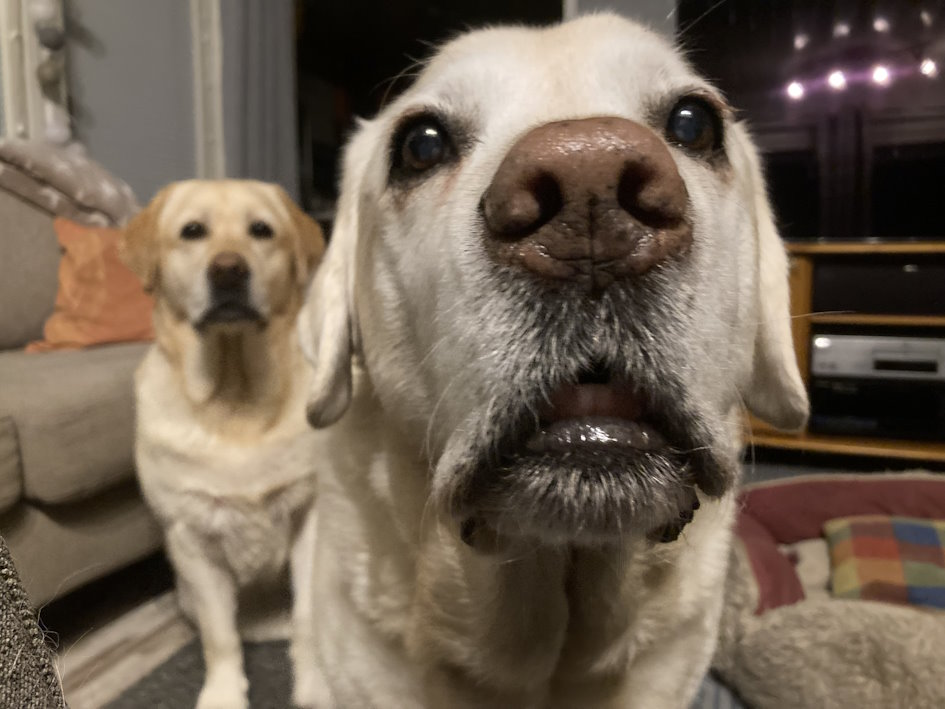
\includegraphics[height=3cm, draft]
    {pictures/TheDogs.jpg}
\end{VerbatimOut}
\ShowExample

\bigskip\noindent%
\emph{What type of file should your graphics be?}
Nowadays the choice is between essentially three formats:\index{pictures!file type}
\begin{description}
\item[PDF] For vector graphics like graphs and line art.
    Vectorized graphics can be zoomed without blurring
    and embedded text is still selectable.

    However, for very complicated graphics
    (say, a scatter plot with 1000 points and transparency),
    it might be better to use a rasterized format.
    PDF graphics are rendered on the reader's device,
    so on a slow device the picture can take a while to load!
\item[PNG] For complex line art.
    PNG is a lossless format, meaning that the picture is reproduced pixel-perfectly.
    The compression algorithm is designed for computer graphics
    with solid colors and simple gradients.
    It is not suitable for photographs (due to massive file sizes).
\item[JPEG] For photographs.
    The algorithm is lossy, meaning that compression artifacts can be seen when zoomed in.
    The artifacts are hard to see in photographs,
    but are very distinguishable in line art and text.

    The algorithm can be set to various compression levels.
    You should experiment with your particular picture,
    but values between 80--90 usually yield a good balance between quality and file size.
\end{description}


\bigskip\noindent%
\emph{What size should the picture be?}\index{DPI}\index{dots per inch!\see{DPI}}
To answer this, we need to talk about DPI -- dots per inch.
Computer screens have something between 100~to 300~pixels per inch.
The standard for printed documents is usually 300~dots per inch,
and up to 600~dpi for high-quality line art.

This means that if your image will be printed 5~cm wide, its pixel width must be at least
\[
\frac{5~\text{cm}}{2.54~\text{cm/in}} \times 300~\text{pixels/in}
= 590~\text{pixels}.
\]
Conversely, the pixel width should not be much larger than this:
the extra resolution would only be seen at very large zoom levels.
\LaTeX{} does not rescale images to a reasonable DPI value,
so extra-large images cause the final document to have larger file size.%
\footnote{You might ask whether file sizes matter in the age of terabyte hard drives
and fiber optic internet.
I have downloaded enough many articles onboard long-distance trains
to be allergic to any unnecessary kilobytes.
Fast connections are not universal.}

The PDF format uses inches instead of pixels.
Still, by setting the image size to the correct value you ensure that
text and lines are drawn at a scale matching the rest of the document.


\begin{practices}
To summarize:
\begin{itemize}
\item If it is a photograph, use JPEG with suitable size and compression level.
\item If you're exporting graphics from an application or script,
    set the figure size and DPI to the intended size and export as PDF.
    If PDF is not available or the image file gets very large, use PNG.
\end{itemize}
\end{practices}


\begin{practices}
Avoid screenshots;
always export your graphics directly from the application if possible.
Most operating systems render text with smoothing adapted to your screen
-- the (no longer adapted) smoothing is visible in a screenshot.

In particular, Windows uses a sub-pixel rendering algorithm
that is very visible as coloured artifacts around black text.
\end{practices}


\begin{latexthree}
Since late~2021, \cmd[alt text]{includegraphics}\index{pictures!alt text}
has also supported setting \emph{alt text}: a textual description of the image.
It is passed as the optional \verb|alt| parameter;
see the example on page~\pageref{ex:alt text}.
This text is used when the document is read aloud by a screen reader program.

The alt text should give enough information to understand the message in the image.
Writing good alt text is not easy,
but there are some resources online.
For some examples, see the decision tree and links therein by W3C\footnotemark.
\end{latexthree}
\footnotetext{\url{https://www.w3.org/WAI/tutorials/images/decision-tree/}.
The WWW Consortium maintains web standards, so parts of the tutorial are web-specific.}



%
%
%
\section{Floats}\label{sec:floats}

Numbered figures and tables in \LaTeX{} are collectively known as \emph{floats}.%
\index{floats}\index{figures}%
\footnote{Named after their tendency to float around into inconvenient places.}
The algorithm to place floats is again very complicated,
with some 20~tunable parameters;
these are explained in detail in \cite[Chapter~7.1]{TLC}.

A rough summary of the rules is:
\begin{itemize}
\item Floats can appear inline, at the top or bottom of the page, or on a separate page.
    The possible locations are preset by the document class
    and can be restricted in the code.
    In two-column mode, there is also the top of page spread across the two columns.
\item Floats are always placed in order within a float class.
    That is, Figure~1 always appears before Figure~2 and Table~1 before Table~2.
    However, tables and figures are placed independently,
    so their order with respect to each other might be anything.
\item \LaTeX{} first tries to put the float on the page where the surrounding code is set.
    If that fails, the float goes into a queue to be reconsidered for the next page.
    Consequently, a float might appear above the surrounding text on the same page,
    but never on an earlier page.
\item \LaTeX{} might produce one or more pages containing only floats if the queue is full enough.
\item At the end of document, all remaining unplaced floats are printed.
\end{itemize}

To override the float placement, you can put one or more letters in an optional argument
after the \verb|\begin{figure}| (or similar) command.
These specifiers \emph{exclude} the unmentioned specifiers,
so defining this always restricts \LaTeX's opportunities.
\begin{description}
\item[\texttt{t}] Allow putting the float at top of page.
\item[\texttt{b}] Allow putting the float at bottom of page.
\item[\texttt{p}] Allow putting the float on a separate page.
\item[\texttt{h}] Tries to put the float inline at the given position.
    If there is not enough space, the specifier is converted to \verb|t|.
\item[\texttt{!}] Ignores certain restrictions about the number of floats on a single page.
\end{description}
%
Quite often the default is \verb|tbp|, which corresponds to what is usually considered good style.
You can use \verb|h| to suggest placing the float inline, but it might still appear
at the top of next page.
If you really need to force an inline float (and most probably you should not),
you can load the \pkg{float} package and use its \verb|H| specifier.

Sometimes the algorithm leads to very many float pages that consist of mainly whitespace.
If you are in control of the document layout,
then the \pkg{fewerfloatpages} package might be useful.
Its documentation also contains some more explanation of the placement algorithm.

\begin{practices}
As with overfull lines, you should not tweak the placement of floats until at the very end.
Small changes to the text might change the page layout significantly.
Unless you get a visually unpleasing arrangement, avoid adding placement restrictions.
\end{practices}

\begin{gotcha}
Due to the algorithm, there are a few surprising things:
\begin{itemize}
\item The order of placement specifiers is irrelevant;
    \LaTeX{} always evaluates its options in the order ``here''--``top''--``bottom''--``queue it''.
\item In two-column mode, \verb|b| has no effect
    unless bottom-of-column floats are allowed with a special package.
    If \verb|b| is the only placement specifier, this ensures that your float will not be set!
\item In some rare cases, the placement of floats might push footnotes into an incorrect page.
\end{itemize}
\end{gotcha}

Figure captions are generated with the \cmd{caption} command.
This command also updates the figure number,
so a possible cross-reference \cmd[figures]{label} must come after it.

As a complete example, \Cref{fig:cira} is produced with the following code.
The specifier \verb|[ht]| forces \LaTeX{} to put the figure either immediately
after this paragraph or on top of a following page; it cannot appear at the bottom of a page.
It is usually customary to center the figure,
which is done with the \cmd{centering} command that applies until the environment ends.%
\label{ex:alt text}
%
\begin{VerbatimOut}{\jobname.tmp}
\begin{figure}[ht]
\centering
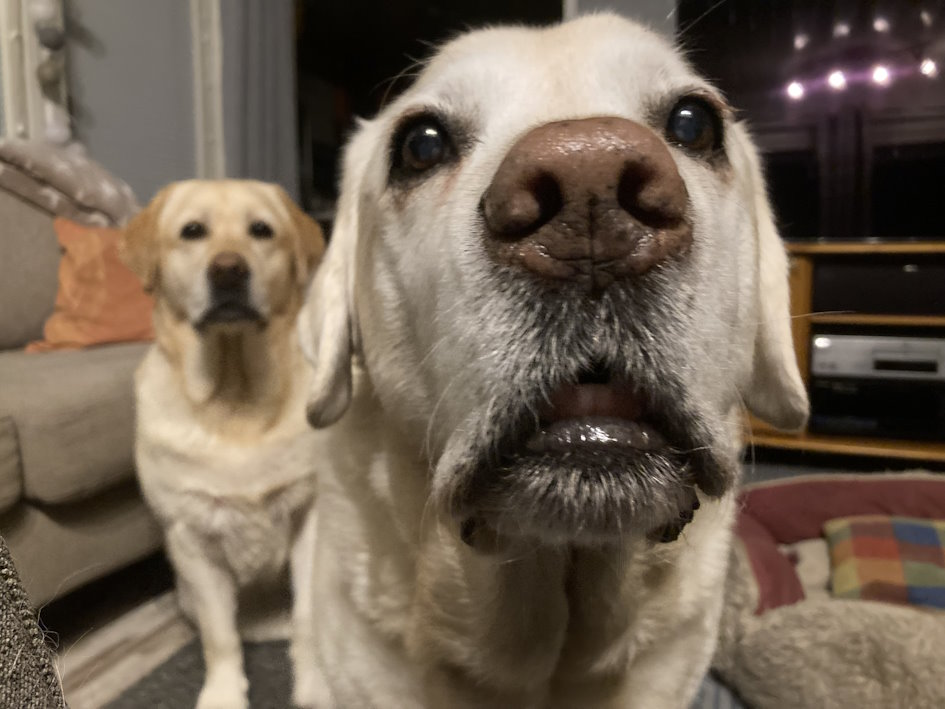
\includegraphics[width=8cm,
  alt={An old labrador retriever close up,
    with intense gaze and mouth slightly open.
    In the background, a younger labrador also stares at the camera.}]
  {pictures/TheDogs.jpg}
\caption{Cira (2009--2022) having a say.}
\label{fig:cira}
\end{figure}

\end{VerbatimOut}
\ExecuteExample

It is possible to print a list of figures\index{figures!list of}
with the \cmd{listoffigures} command.
This command requires one extra run of the compiler in order to be in sync with the document.
If your figure caption is very long,
you can specify a shorter version for the list in an optional argument:%
\footnote{Akin to the sectioning commands and table of contents.}
\begin{ExampleCode}
\caption[An old labrador]{Cira (2009--2022) having a say.}
\end{ExampleCode}


%
%
\subsection{Subfigures}

Floats are just containers for arbitrary \LaTeX{} code,
so in principle you are free to put anything in there, even text.
This can be abused to create subfigures as in \Cref{fig:hacky subfigs}:
%
\begin{VerbatimOut}{\jobname.tmp}
\begin{figure}
\centering

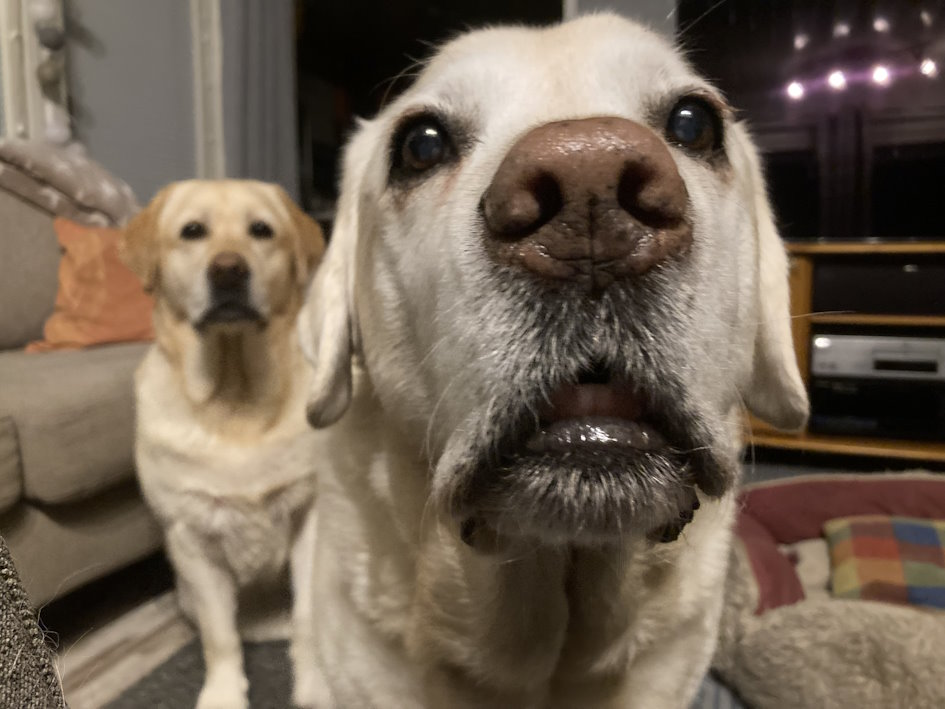
\includegraphics[width=0.4\textwidth, alt={The two dogs.}]
  {pictures/TheDogs.jpg}
\hspace{1em}
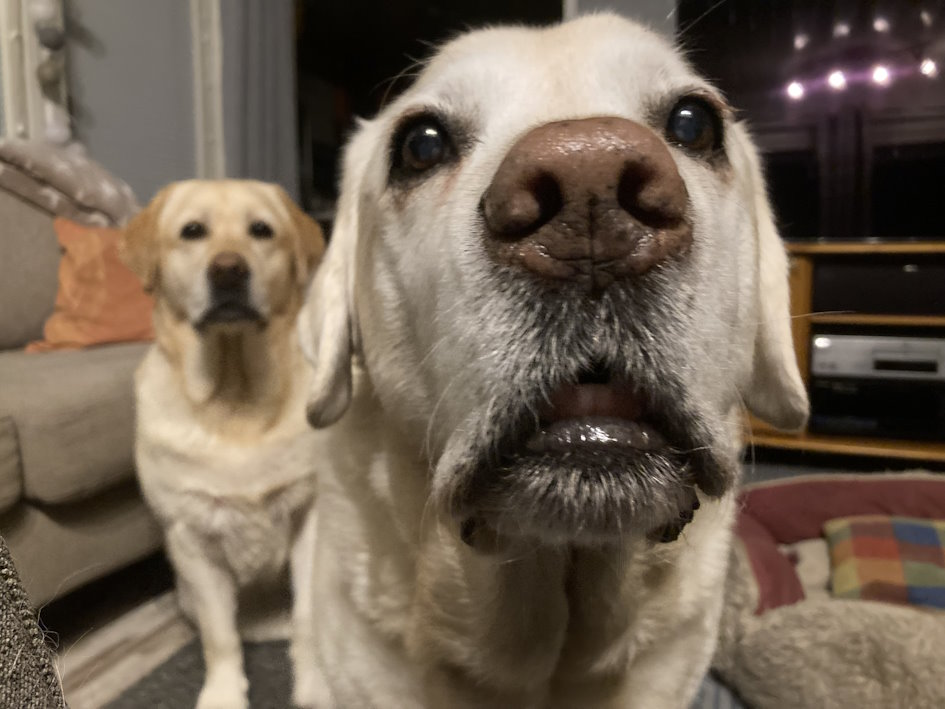
\includegraphics[angle=180, origin=c,
    width=0.4\textwidth, alt={Same dogs upside down.}]
  {pictures/TheDogs.jpg}

\caption{Left: some dogs. Right: some upside-down dogs.}
\label{fig:hacky subfigs}
\end{figure}

\end{VerbatimOut}
\ExecuteExample

However, there is also the \pkg{subcaption} package that does the same automatically
and with more style.

\begin{warning}
Do not use the \obspkg{subfigure} or \obspkg{subfig} packages;
they are no longer maintained and do not play as well together with
\pkg[problematic packages]{hyperref}.
\end{warning}

This package offers the \cmd{subcaptionbox} that takes 2--5 arguments:
optional short caption, the caption, optional width for the subfigure,
optional alignment for the subfigure (\verb|l|, \verb|c|, or \verb|r|),
and finally the figure contents.

\Cref{fig:subcaption} shows how this looks in practice.
Note how the lines of figures need to be broken by a paragraph break (empty line);
one could put a vertical spacing command here.
For the third subfigure (\Cref{fig:subcaption small dog}),
the width is set manually so that the caption is not broken into two lines.
Note that \cmd[subfigures]{label} can be used, but it needs to be inside the caption argument.%
\footnote{To reference the subfigure letter without the main figure number,
the package provides a \cmd{subref} command.}
%
\begin{VerbatimOut}{\jobname.tmp}
\begin{figure}
\centering

\subcaptionbox{As usual.}{
  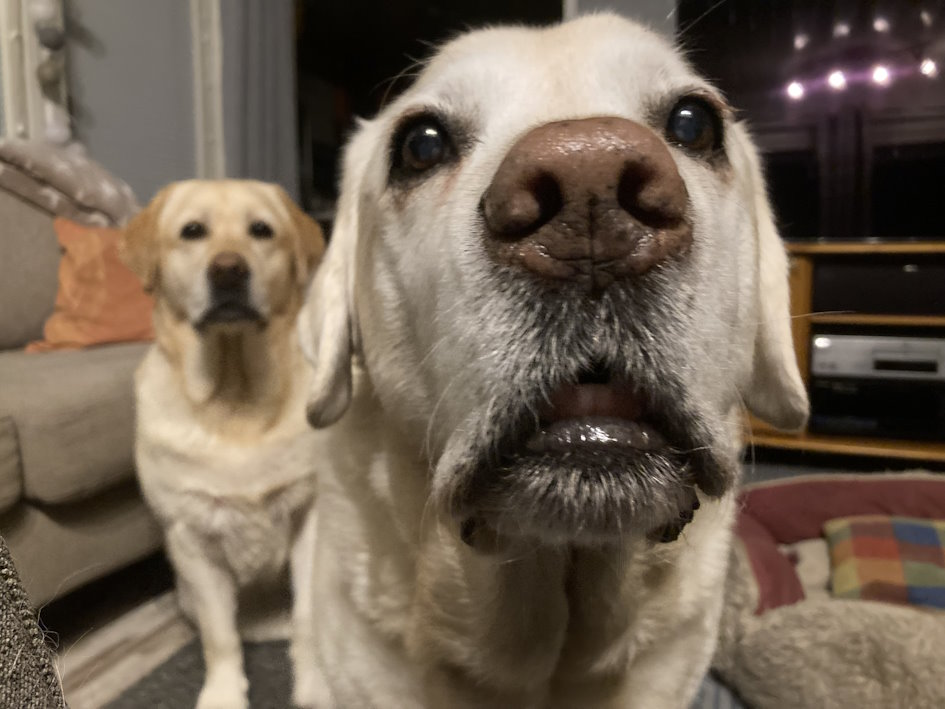
\includegraphics[width=0.4\textwidth]{pictures/TheDogs.jpg}}
\subcaptionbox{Upside down.}{
  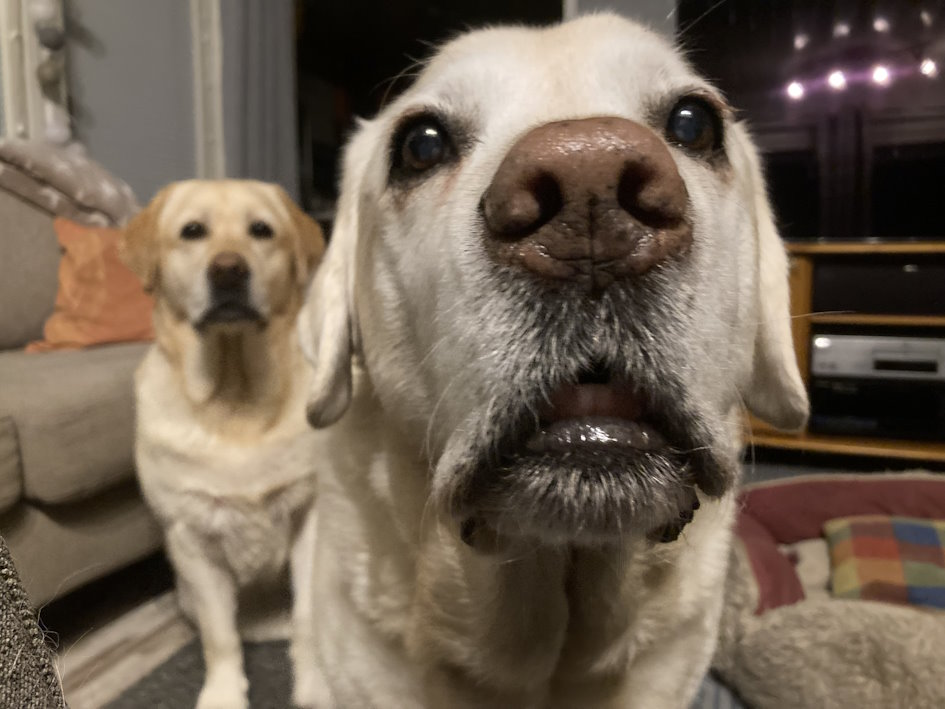
\includegraphics[angle=180, origin=c, width=0.4\textwidth]
    {pictures/TheDogs.jpg}}

\subcaptionbox{The smaller one.\label{fig:subcaption small dog}}[3cm]{
  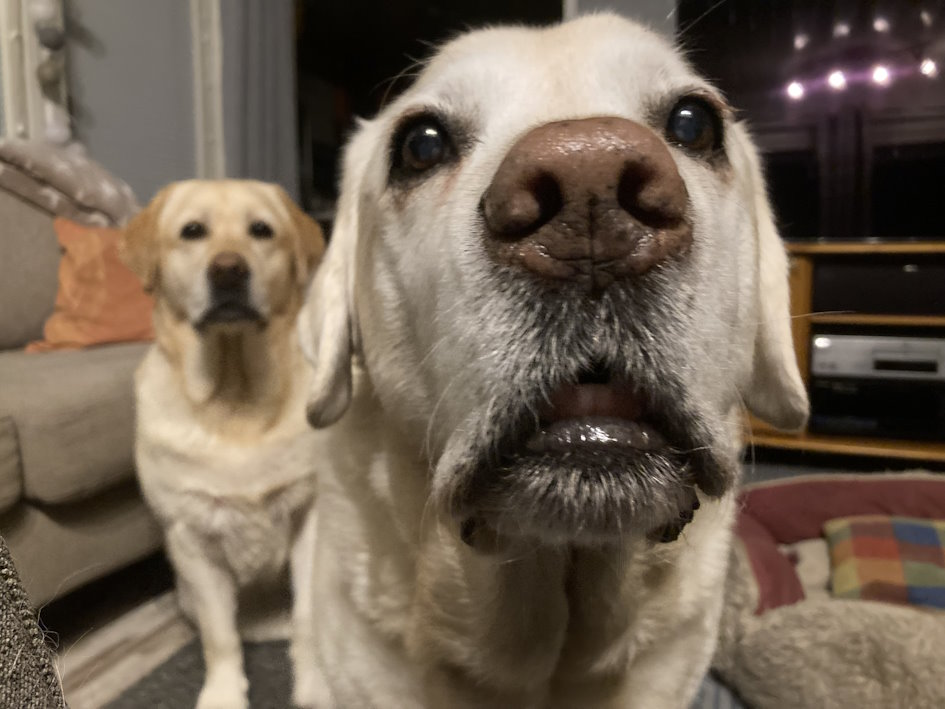
\includegraphics[bb=1cm 2cm 3cm 5cm, clip]
    {pictures/TheDogs.jpg}}
\subcaptionbox{The larger one.}{
  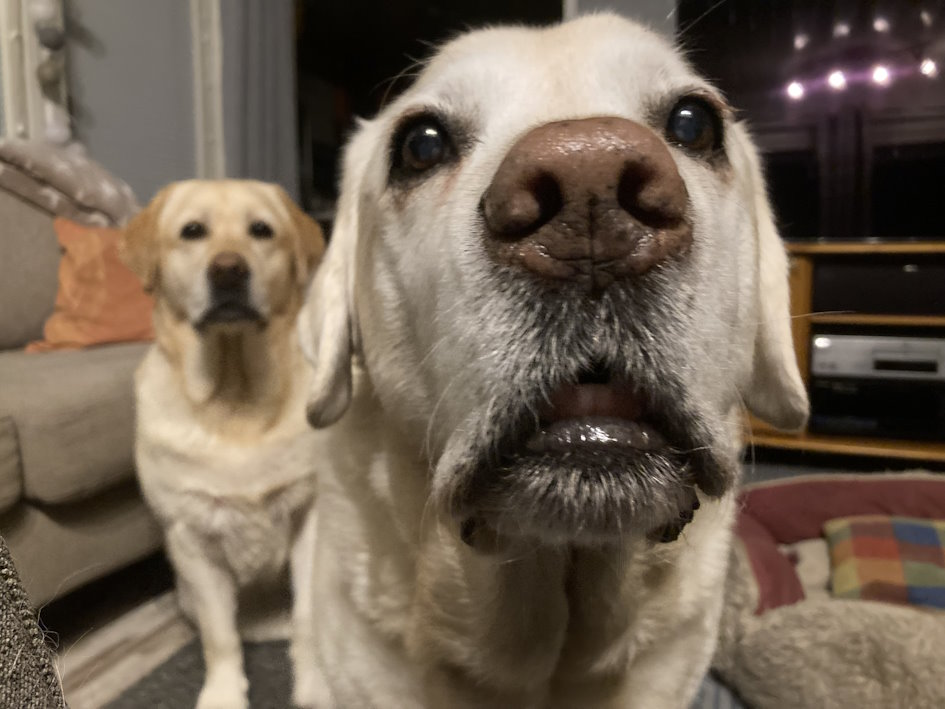
\includegraphics[bb=2.8cm 1.4cm 7cm 6cm, clip, scale=0.8]
    {pictures/TheDogs.jpg}}
\subcaptionbox{Right-aligned and fixed width.}[3.5cm][r]{
  \scshape Lorem ipsum dolor sit amet.}

\caption{A collection of dogs and a typographical example sentence.}
\label{fig:subcaption}
\end{figure}
\end{VerbatimOut}
\ExecuteExample


%
%
\subsection{Custom float environments}\label{sec:custom floats}

By default, \LaTeX{} provides the \env{figure} and \env{table} environments
and the corresponding commands for lists of figures and tables.
It is possible to also introduce new float environments with the \pkg{float} package.
This is useful for e.g.\ source code listings.

The \cmd{newfloat} command takes 3--4~arguments:
the environment name to use,
the default placement specifier (remember that the default is usually \verb|tbp|),
file name extension for the auxiliary file (must not be already in use!),
and optionally the number-within level.

To customize the look of the new float,
a \cmd{floatstyle} command can be put before the definition.
By default there are four options: \verb|plain|, \verb|plaintop| (caption on top),
\verb|boxed|, and \verb|ruled|.
The displayed name of the new environment can be set with the \cmd{floatname} command.

For example, a float class for source code listings could be defined as follows.
(Note: the \pkg{listings} package also has an option to define a float class,
so it is not necessary to do this manually.)
%
\begin{VerbatimOut}{\jobname.tmp}
\floatstyle{ruled}
\newfloat{sourcecode}{tbp}{lst}[chapter]
\floatname{sourcecode}{Code Listing}
\end{VerbatimOut}
\ExecuteExample  

It would then produce a float like Code~Listing~\ref{src:hello pascal}.
%
\begin{VerbatimOut}{\jobname.tmp}
\begin{sourcecode}[h]
\begin{lstlisting}[language=Pascal]
program Hello;

begin
writeln("Hello world!");
end.
\end{lstlisting}
\caption{A Hello World program in Pascal.}
\label{src:hello pascal}
\end{sourcecode}
\end{VerbatimOut}
\ExecuteExample


%
%
\subsection{Landscape floats}\label{sec:landscape floats}

\todo{Especially useful for tables}


%
%
\subsection{Customizing captions}

\todo{Starred command}

\todo{Is this actually necessary?}



%
%
%
\section{Creating tables}

The \env{tabular} environment offered by \LaTeX{} is sufficient for simple tables.
It consists of table contents and certain special elements:
\begin{itemize}
\item In the beginning, there is a \emph{column specification}.
    The number of columns is fixed here, and for each column the alignment of text is indicated:
    \verb|l| for left-aligned, \verb|c| for centered, and \verb|r| for right-aligned.
    Fixed width can be given with \verb|p{...}|.

    Additionally, vertical lines can be specified with \verb+|+ and
    other inter-column material with \verb|@{...}|.
\item On each line, columns are separated by \verb|&|.
\item Each line is ended with \verb|\\|.
    If you forget to end a line, you will get an error at the next \verb|&|.
\item Horizontal lines can be created with \verb|\hline|.
    No \verb|\\| is then necessary.
\end{itemize}
%
Let us illustrate these with a simple example:
%
\begin{VerbatimOut}{\jobname.tmp}
\begin{tabular}{l| c p{3cm} c @{ $\Rightarrow$ } r}
Breed & Drops fur & Notes & Rating & Conclusion\\
\hline
Corgi & Somewhat & Has fairly short legs but a lot of attitude
    & 13/10 & Good dog\\
Labrador & Very much & Excitable about other dogs, humans, playing in water
    & 13/10 & Good dog
\end{tabular}
\end{VerbatimOut}
\ShowExampleBelow

The \env{table} environment acts exactly like its figure counterpart,
and should be used for tables where the exact placement is not so important.
The following code produces \Cref{tbl:dogs}:
%
\begin{VerbatimOut}{\jobname.tmp}
\begin{table}[ht]
\centering
\begin{tabular}{l|ccc}
  Breed & Drops fur & Tall & Long\\
  \hline
  Corgi & Somewhat & Very not & Quite\\
  Labrador & Very much & Yes & Yes
\end{tabular}
\caption{An extensive comparison of dog breeds.}
\label{tbl:dogs}
\end{table}
\end{VerbatimOut}
\ExecuteExample


If you need more customization for your tables, then the \pkg{array} package is the starting point.
First off, it adds the following format specifiers:
\begin{description}
\item[\texttt{m}] Fixed-width column like \verb|p|, but centered vertically.
\item[\texttt{w}] This takes two parameters: alignment and width.
    There is \emph{no} automatic line breaking,
    so the contents may overprint adjacent cells!
\item[\texttt{W}] Like above, but tries to squeeze the text a bit and if still fails,
    at least raises an overfull hbox warning.
\item[\texttt{>}] Takes one argument, which is inserted in front of each entry.
\item[\texttt{<}] Like above, but after the entry.
\item[\texttt{!}] Like the \verb|@| specifier,
    but preserves the horizontal space that would surround a vertical line.
\end{description}

The previous example can be customized as follows.
We use the \verb|>| and \verb|<| specifiers to set the rating in a bold font
and to remove the duplicated \verb|/10| texts.
Since \verb|!| preserves the whitespace,
we no longer need spaces around the arrow symbol.
%
\begin{VerbatimOut}{\jobname.tmp}
\begin{tabular}{l| c m{3cm} >{\bfseries}c<{/10} !{$\Rightarrow$} r}
Breed & Drops fur & Notes & Stars & Conclusion\\
\hline
Corgi & Somewhat & Has fairly short legs but a lot of attitude
    & 13 & Good dog\\
\hline
Labrador & Very much & Excitable about other dogs, humans, playing in water
    & 13 & Good dog
\end{tabular}
\end{VerbatimOut}
\ShowExampleBelow
%
Note that the change from \texttt{p} to \texttt{m} does not improve legibility here;
that's why I added a horizontal line to separate the two rows.
There would also be several methods to add vertical whitespace to the table:
\begin{itemize}
\item Optional argument to \verb|\\|:
    however, the value is interpreted as the desired \emph{total height} of the row,
    and not as a skip.
    If the value is smaller than the current height, this has no effect.
\item The \verb|\extrarowheight| length specified by \pkg{array}
    is added to the beginning of each row.
    By default it is \verb|0pt|;
    see the example on page~\pageref{ex:extrarowheight} for a different value.
\item The \pkg{cellspace} package can be used to ensure top and bottom vertical clearances
    when the cell contents are taller than usual characters.
    This package defines a modifier for cell styles.
\end{itemize}

\todo{Ragged right in table}


%
%
\subsection{Special cells}

If you need a cell to span several columns,
you can use the \cmd{multicolumn} command.
It takes three arguments: the number of columns to extend to,
a new column specification for the internal contents, and finally the contents.\label{ex:extrarowheight}
%
\begin{VerbatimOut}{\jobname.tmp}
\setlength\extrarowheight{2pt}
\centering
\begin{tabular}{l| c c @{ $\Rightarrow$ } r}
Breed & Drops fur & Rating & Conclusion\\
\hline
Corgi & Somewhat & 13/10 & Good dog\\
Labrador & Very much & 13/10 & Good dog\\
Roomba & Negatively?! &
    \multicolumn{2}{c}{\emph{We're not quite sure}}
\end{tabular}
\end{VerbatimOut}
\ShowExampleBelow
%
In this example, the last two columns (specified \verb|c r|)
were replaced by a single \verb|c| cell.

To use colours, one can use the \pkg{colortbl} package.
Remember to use colour only moderately and to maintain a good colour contrast.
(The following example fails at any artistic merits for illustrative purposes.)
%
\begin{VerbatimOut}{\jobname.tmp}
\centering
\begin{tabular}{>{\columncolor{green!15}}l | c c @{ $\Rightarrow$ } r}
\rowcolor{blue!15} Breed & Drops fur & Rating & Conclusion\\
\hline
Corgi & Somewhat & 13/10 & Good dog\\
Labrador & Very much & 13/10 & Good dog\\
Roomba & \cellcolor{orange!20} Negatively?! &
    \multicolumn{2}{c}{\emph{We're not quite sure}}
\end{tabular}
\end{VerbatimOut}
\ShowExampleBelow
%
Here the \cmd{columncolor} command goes into the column specifier, and
the \cmd{rowcolor} command goes into the beginning of each row.
As you can see, the latter is not fully compatible with custom separators.
As each cell forms a scope, you can also use \cmd[in table]{color} to set the text color in a cell.

The \pkg{diagbox} makes it possible to split cells diagonally.
It has quite a lot of configuration options as optional arguments,
but we refer the reader to the package documentation.
It also has a somewhat esoretic syntax that accepts \emph{two or three} required arguments,
meaning that the two-argument version cannot be followed by a \verb|{|.
(This is quite unlikely in a table cell.)
%
\begin{VerbatimOut}{\jobname.tmp}
\centering
\begin{tabular}{l|ccc}
  \diagbox{Breed}{Property} & Drops fur & Tall & Long\\
  \hline
  Corgi & Somewhat & Not & Quite\\
  Labrador & Very much & Yes & Yes\\
  Roomba & Negatively & Very not & It's round
\end{tabular}
\end{VerbatimOut}
\ShowExampleBelow



%
%
\subsection{Footnotes in tables}\label{sec:table footnotes}

Finally, let us talk about footnotes in tables,
as sometimes mandated by scientific style.
As discussed in \Cref{sec:footnotes},
\cmd[in tables]{footnote} commands inside a \verb|tabular| environment
do not print the footnote text anywhere.

A simple fix is to place the table inside a \env{minipage} environment.
Often, an easier alternative is to use the \pkg{threeparttable} package
that provides its own footnote command.
You are required to take care of the numbering,
but this is actually useful since commonly the same footnote is used for several locations.
%
\begin{VerbatimOut}{\jobname.tmp}
\centering
\begin{threeparttable}
\begin{tabular}{l|ccc}
  Breed & Drops fur & Tall & Long\\
  \hline
  Corgi & Somewhat\tnote{a} & Not\tnote{b} & Quite\tnote{b}\\
  Labrador & Very much\tnote{c} & Yes\tnote{b,c} & Yes\tnote{b,c}\\
  Roomba & Negatively\tnote{d} & Very not\tnote{b} & It's round\tnote{b}
\end{tabular}
\begin{tablenotes}[para]
  \item[] Sources:
  \item[a] Googling.
  \item[b] General knowledge.
  \item[c] Having lived with some.
  \item[d] Rumours.
\end{tablenotes}
\caption{Some extensive research into things.}
\end{threeparttable}
\end{VerbatimOut}
\ShowExampleBelow


If you ever need to set a table that spans multiple pages,
the \pkg{supertabular} and \pkg{longtable} packages are your friends.
The first one is simpler but the second is more extensible and more maintained.



%
%
\subsection{Final words}

There are several more useful packages for controlling the layout of tabular material.
Most mathematicians will probably not need them,
but \cite{TLC} has over 70~pages on this topic if the need arises.

\begin{latexthree}
As of this writing in April~2024,
PDF tagging of tables has recently entered testing.
This means that tables should no longer be completely meaningless jumbles of text and numbers
to a screen reader.

The syntax for annotating tables is still being worked out.
In a future \LaTeX{} version, there should be syntax for annotating column headers.
Follow the news on \LaTeX{} homepage to know what's happening!
\end{latexthree}
